pc\chapter{Discussão}

Nesta seção, são analidos os resultados obtidos a fim de responder as perguntas que motivaram este estudo.

\section{Algoritmos linear mais eficiente}

A primeira pergunta a ser respondida é qual dos dois algoritmos lineares simulados é mais eficiente. Na figura \ref{fig:lvsj_search_time}, estão os resultados da busca linear e da {\it jump search}. Claramente, a {\it jump search} é mais eficiente, chegando a ser mil vezes mais rápida para o maior tamanho de arranjo simulado. Na ampliação mostrada na figura \ref{fig:lvsj_search_time_zoom} podemos observar melhor a diferença de eficiência entre os dois algoritmos. 

\begin{figure}[H]
  \centering
  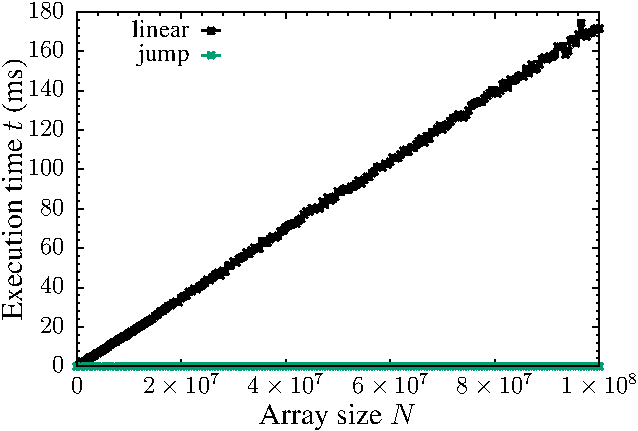
\includegraphics[scale=1.2]{../plots/lvsj_search_time.pdf}
  \caption{Comparação do tempo de execução médio das simuluções dos algoritmos lineares: busca linear (preto) e {\it jump search} (verde).}
  \label{fig:lvsj_search_time}
\end{figure} 

\begin{figure}[H]
  \centering
  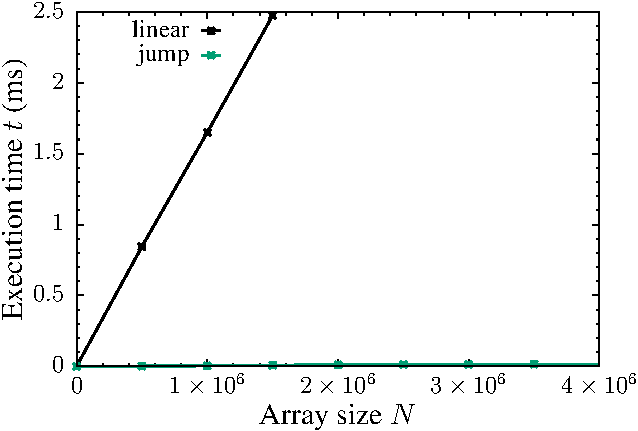
\includegraphics[scale=1.2]{../plots/lvsj_search_time_zoom.pdf}
  \caption{Ampliação da figura \ref{fig:lvsj_search_time}.}
  \label{fig:lvsj_search_time_zoom}
\end{figure} 


\section{Implementação mais eficiente: recursiva ou iterativa?}

O segundo objetivo é determinar qual implementação é mais eficiente, se a recursiva ou a iterativa. Analisando as curvas mostradas nas figuras \ref{fig:bsearch_ivsr_time} e \ref{fig:tsearch_ivsr_time} verifica-se que a versão iterativa e recursiva se diferenciam muito pouco, tanto na versão binária ou ternária do algoritmo. Para alguns tamanhos a curva da implementação iterativa parece ligeiramente mais eficiente, no entanto a medida de tempo de execução está sujeita a flutuações e não há uma medida do erro da obtenção dos pontos por isso fica difícil concluir qual implementação é mais eficiente com esses dados.
\begin{figure}[H]
  \centering
  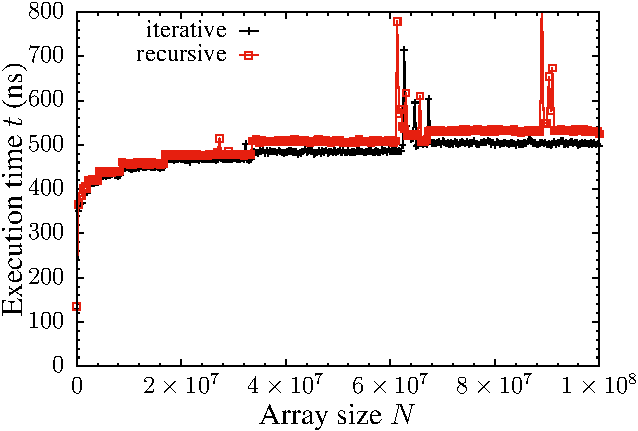
\includegraphics[scale=1.2]{../plots/bsearch_itvsrec_time.pdf}
  \caption{Comparação do tempo de execução médio das simuluções da implementação iterativa (preto) e recursiva (vermelho) do algoritmo de busca binária.}
  \label{fig:bsearch_ivsr_time}
\end{figure} 

\begin{figure}[H]
  \centering
  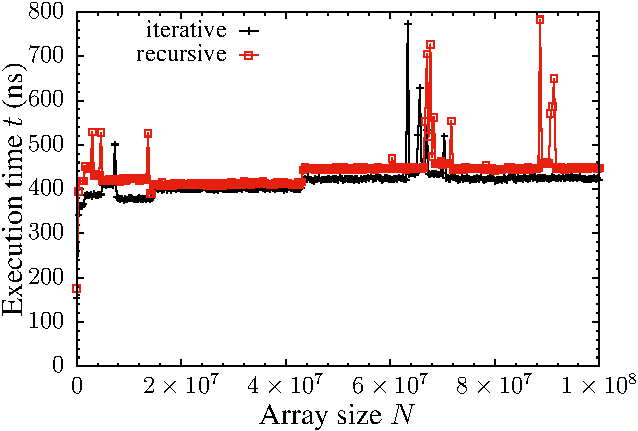
\includegraphics[scale=1.2]{../plots/tsearch_itvsrec_time.pdf}
  \caption{Comparação do tempo de execução médio das simuluções da implementação iterativa (preto) e recursiva (vermelho) do algoritmo de busca ternária.}
  \label{fig:tsearch_ivsr_time}
\end{figure} 


\section{Influência do tamanho da partição nos algoritmos de busca não lineares}

Outra comparação interessante pode ser feita com os algoritmo de busca binária e ternária (figura \ref{fig:bvstvsfib_search_time}). Assim consegue-se verificar a influência do tamanho da partição nas buscas não lineares. Dos dados obtidos, pode-se concluir que a busca ternária é ligeiramente mais rápida que a binária.

\begin{figure}[H]
  \centering
  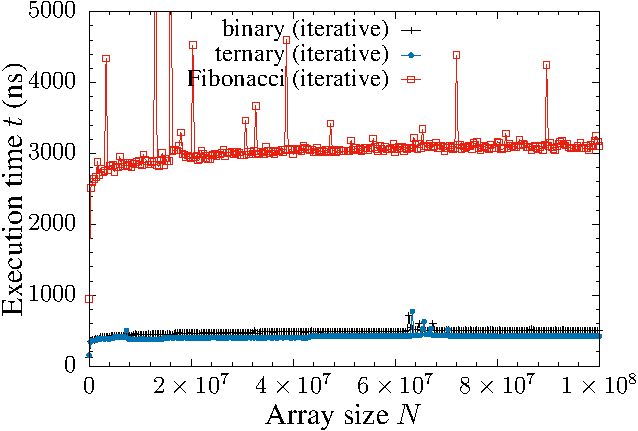
\includegraphics[scale=1.2]{../plots/bvstvsfib_search_time.pdf}
  \caption{Comparação entre algoritmos (versões iterativas) com diferentes tamanhos de partições: binário (preto) e ternário (azul).}
  \label{fig:bvstvsfib_search_time}
\end{figure} 


\section{Diferenciação de algoritmos de classe de complexidade diferentes}

Como pode ser verificado na seção de resultados, para tamanhos grandes do arranjo, enquanto a busca linerar demora centenas de milisegundos, a busca binária demora centenas de nanosegundos (10$^6$ vezes menos), sendo consideravelmente mais eficiente. Uma pergunta relevante nesse caso, é a partir de que momento algoritmos de classe de complexidade diferentes se diferenciam. Comparando a busca linear com a binária (figura \ref{fig:lvsb_search_time}), concluímos que para tamanhos superiores que 100 a busca binária já é superior.

\begin{figure}[H]
  \centering
  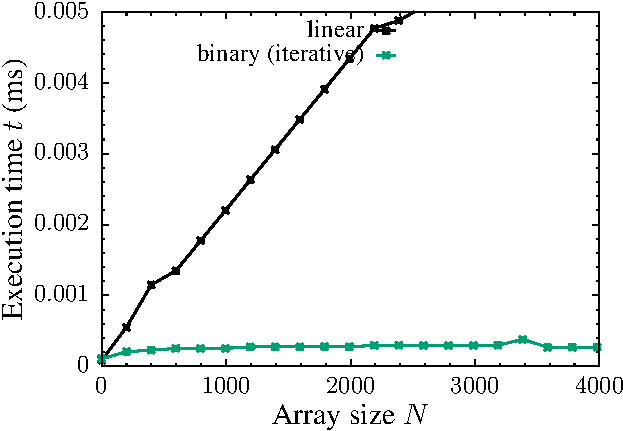
\includegraphics[scale=1.2]{../plots/lvsb_search_time.pdf}
  \caption{Comparação do tempo de execução médio da busca linear (preto) com a binária (verde).}
  \label{fig:lvsb_search_time}
\end{figure} 

%\section{Cenários do algoritmo de Fibonacci}
%
%Por fim, o quinto objetivo procura determinar se existe diferentes categorias de cenários de pior caso para o algoritmo de busca de Fibonacci.
%
%\begin{figure}[H]
%  \centering
%  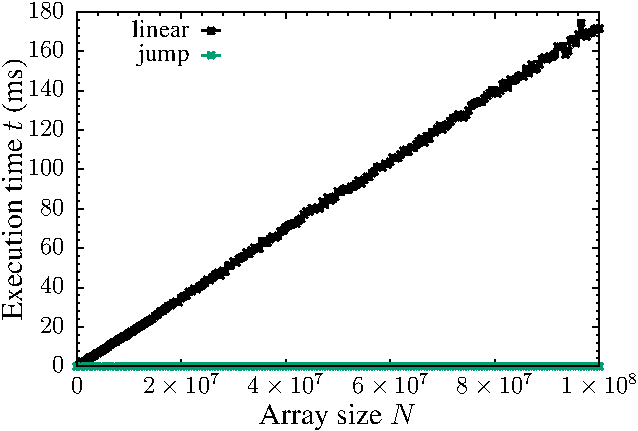
\includegraphics[scale=1.2]{../plots/lvsj_search_time.pdf}
%%  \caption{Comportamento assintótico da {\it jump search} em relação ao tempo de execução médio (medido em milisegundos) a medida que o tamanho do arranjo sequencial $N$ aumenta.}
%\end{figure} \label{fig:lvsj_search_time}
